\documentclass[a4paper,12pt]{article}
\usepackage{amssymb,amsthm}
\usepackage{amsmath}
\usepackage{setspace}
\usepackage{graphicx}
\usepackage{qtree}
\usepackage{xcolor}
\usepackage{tikz}
\usepackage{setspace}
\doublespacing

\usetikzlibrary{automata,positioning,decorations.markings,arrows}
\begin{document}
\newpage
\textbf{Question 1}\\Hosts A and B are each connected via two routers R 1 and R 2 and a with 10 8 bits per
second links. Each link has a propagation delay of 120 microseconds. Processing delay at
router is 500 microseconds.\\\\
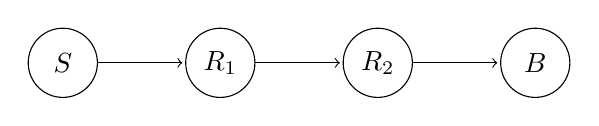
\begin{tikzpicture}[shorten >=1pt,node distance=2cm,on grid,auto]
  \node[state] (A)      {$S$};
  \node[state]         (R1) [right of=A]  {$R_1$};
  \node[state]         (R2) [right of=R1] {$R_2$};
  \node[state]         (B) [right of=R2] {$B$};
  \path[->]  (A)  edge              node {} (R1);
  \path[->]  (R1)  edge              node {} (R2);
  \path[->]  (R2)  edge              node {} (B);
\end{tikzpicture}\\\\
If message size is 10 KB.Calculate the time elapsed between the transmission of the first
bit of data and the reception of the last bit of the data in the following cases :\\

$ (a) $ If message switching technique is used.\\

$ message switching: t_{t}=\dfrac{message size}{data rate}$\\ 
$ t_{t}=\dfrac{10*1024*8}{10^{8}}=819.2us$\\

$ the message at r_{1} t_{1}=t_{t}+120us$\\\\
$ r_{1} t_{1}=819.2+120=839.2us$\\\\
$ the message at r_{2} t_{2}=t_{1}+500 + t_{t} +t_{t}$\\\\
$ the message at B t_{3}=t_{2} + 500 + 120 + 819.2$\\\\
$ T =3817.2 us $\\\\
 
$ T = 3t_{t} + t_{p_{r1}} + t_{p} + t_{p_{r2}} + t_{p} + t_{p}$\\
$ T = 3t_{t} + 2t_{p} + 3t_{p} $\\
$ T = 3*819+2*500+3*120=3817 us $\\\\

$ (b) $ Assume packet header size is negligible .\\\\
i) $ If packet switching technique is used and 8 packets of same size are used.$\\
$ T = t_{t}+t_{p}+t_{p_{R1}}+t_{p}+t_{t_{1}}+t_{p_{R2}}+t_{p}+t_{t_{1}} $\\

$ packet size =\dfrac{10*1024*8}{8}=10240 bits$\\
$ t_{t1}=\dfrac{10240}{10^{8}}=102.4 us$\\

$ T =819.2+120+500+120+102.4+500+120+102.4=2384 us $\\

ii)$ If packet switching technique is used and 32 packets of same size are used. $\\
$ packet size =\dfrac{10*1024*8}{32}=2560 bits $\\
$ t_{t_{1}}=\dfrac{2560}{10^{8}}=25.6 us $\\

$ T = t_{t}+3t_{p}+2t_{p}+2t_{1} $\\
$ t = 819.2+3*120+2*500+2*25.6=2230.4 us $\\


iii)$ If packet switching technique is used and 64 packets of same size are used. $\\

$ packet size =\dfrac{10*1024*8}{64}=1.280 bits $\\
$ t_{t_{1}}=\dfrac{1.280}{10^{8}}=12.8 us $\\
$ T = t_{t}+3t_{p}+2t_{p}+2t_{1} $\\
$ t = 819.2+3*120+2*500+2*12.8=2179.2 us $\\



$ (C) $ Assume packet header size is 200 bits

i) $ If packet switching technique is used and 8 packets of same size are used.$\\


$ packet size =10240+200=10440 bits $\\
$ t_{t_{1}}=\dfrac{10440}{10^{8}}104.4us and t_{t}=104.4*8=835.2 us $\\
$ T = t_{t}+2t_{p}+3t_{p}+2t_{t1} $\\
$ t = 835.2+2*500+3*120+2*104.4=2.404 us $\\


i) $ If packet switching technique is used and 32 packets of same size are used.$\\


$ packet size =2560+200=2760 bits $\\
$ t_{t_{1}}=\dfrac{2760}{10^{8}}=27.6 us and t_{t}=27.6*32=883.2 us $\\
$ T = t_{t}+2t_{p}+3t_{p}+2t_{t1} $\\
$ t = 883.2+2*500+3*120+2*27.6.4=1415.2 us $\\



i) $ If packet switching technique is used and 64 packets of same size are used.$\\

$ packet size =1280+200=1480 bits $\\
$ t_{t_{1}}=\dfrac{1480}{10^{8}}=14.8 \\us and t_{t}=14.8*64=947.2 us $\\
$ T = t_{t}+2t_{p}+3t_{p}+2t_{t1} $\\
$ t = 947.2+2*500+3*120+2*14.8=1389.6 us $\\




 \textbf{Question 3}\\ Hosts A and B are each connected via router R 1 and a with 5MBps links. Each link has a
propagation delay of 5 milliseconds/KM. Processing delay at router is 400 milliseconds .


\begin{tikzpicture}[shorten >=1pt,node distance=2cm,on grid,auto]
   \node[state] (A) [right=of R1] {$R1$};
   \node[state] (R1) [right=of R1] {$q_2$};
  \path[->]   (A)(R1);
   \path[->]     (R1)(B);
\end{tikzpicture}\\\\


If message size is 100KB .Calculate the time elapsed between the transmission of the first
bit of data and the reception of the last bit of the data in the following cases :
$ (a) $ If message switching technique is used.\\

 $ t_{t}=19.5 ms $\\
$ data =100*8=800 kbits$\\
$ data rate=5*1024*8=40960kb/s $\\

$ t_{t}= \dfrac{data}{data rate}=\dfrac{800}{40960}=19.5 us $\\
$ =2t_{t} +t_{p}+t_{p} $\\
$ t_{p}=30*5+40*50=350 ms=400us $\\
$ T =2*19.5+350+400=789 us$\\


$ (b)$ Assume packet header size is negligible.\\

i) $If packet switching technique is used and 4 packets of same size are used $\\

$ packet size =\frac{800}{4}=200kbits $\\
$ t = T_{t}+t_{p}+t_{p}+t_{t1}$\\
$ t_{t1}=\dfrac{data}{data rate}=\dfrac{200}{40960}=4.88 ms $\\
$ T = 19.5+350+400+4.88=774.38ms $\\

ii) $If packet switching technique is used and 64 packets of same size are used $\\

$ packet size =\frac{800}{64}=12.5kbits $\\
$ t = T_{t}+t_{p}+t_{p}+t_{t1}$\\
$ t_{t1}=\dfrac{data}{data rate}=\dfrac{12.5}{40960}=0.3 ms $\\
$ T = 19.5+350+400+0.3=769.8ms $\\


iii) $If packet switching technique is used and 128 packets of same size are used $\\

$ packet size =\frac{100}{128}=0.78125kb $\\
$ t = T_{t}+t_{p}+t_{p}+t_{t1}$\\
$ t_{t1}=\dfrac{data}{data rate}=\dfrac{0.78125}{5.20}=0.15 ms $\\
$ T = 19.5+350+400+0.15=768.65ms $\\\\




$ (c)$ Assume packet header size is 400 bits\\
i)$ If packet switching technique is used and 4 packets of same size are used. $\\

$ message size is 100*1024=102400 b $\\
$ packet size=\dfrac{message size}{packet}+header=\dfrac{102400}{4}+400=26000 bits $\\
$ t = T_{ti}+t_{p}+t_{p}+t_{t1}$\\
$ t_{t1}=\frac{26000}{5*2^{20}}=4.95 and t_{ti}=4.95*4=19.8 ms $\\
$ T = 19.8+350+400+4.95=774.75 ms $\\

ii)$ If packet switching technique is used and 64 packets of same size are used. $\\

$ message size = 81900 $\\
$ packet size=\dfrac{message size}{packet}+header=\dfrac{819200}{64}+400=13200 bits $\\
$ t = T_{tii}+t_{p}+t_{p}+t_{t1}$\\
$ t_{t1}=\frac{13200}{5*2^{20}*8}=0.31 and t_{tii}=64*0.31=20.1 ms $\\
$ T = 20.1+350+400+0.31=770.41 ms $\\


iii)$ If packet switching technique is used and 128 packets of same size are used. $\\

$ message size = 81900 $\\
$ packet size=\dfrac{message size}{packet}+header=\dfrac{819200}{128}+400=6800 bits $\\
$ t = T_{tiii}+t_{p}+t_{p}+t_{t1}$\\
$ t_{t1}=\frac{6800}{5*2^{20}*8}=0.16 and t_{tiii}=128*0.16=20.7 ms $\\
$ T = 20.7+350+400+0.16=770.9 ms $\\



\textbf Q5. Hosts A and B are each connected via three routers R 1 , R 2 and R 3 and a with 5MBps
links. Each link has a propagation delay of 500 millisecond/KM. Processing delay at
router is 500 microseconds.\\

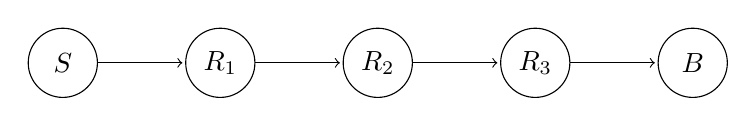
\begin{tikzpicture}[shorten >=1pt,node distance=2cm,on grid,auto]
  \node[state] (A)      {$S$};
  \node[state]         (R1) [right of=A]  {$R_1$};
  \node[state]         (R2) [right of=R1] {$R_2$};
  \node[state]         (R3) [right of=R2] {$R_3$};
  \node[state]         (B) [right of=R3] {$B$};
  \path[->]  (A)  edge              node {} (R1);
  \path[->]  (R1)  edge              node {} (R2);
  \path[->]  (R2)  edge              node {} (R3);
  \path[->]  (R3)  edge              node {} (B);
\end{tikzpicture}\\\\

If message size is 100KB .Calculate the time elapsed between the transmission of the first
bit of data and the reception of the last bit of the data in the following cases :


$ (a) $ If message switching technique is used.\\


$ T =t_{t}+t_{p_{r1}}+t_{p_{r1}}+t_{t}+t_{p_{r1-r2}}+t_{p_{r2}}+t_{t}+t_{p_{r2-r3}}+t_{p_{r3}}+t_{t}+t_{p_{r3b}}$\\
$ T =4t_{t}+t_{p}+t_{p}$\\
$ t_{p}=t_{pr_{R1}}+t_{pr_{R2}}+t_{pr_{R3}}=500*300+500*40+500*45+500*60=87500/10^{3}$\\
$ t_{p}=t_{pr_{R1}}+t_{pr_{R2}}+t_{pr_{R3}}+t_{p_{R3B}}=500*300+500*40+500*45+500*60+500*3=131250000*10^{3}$\\
$ t_{t}=\dfrac{data}{data rate}=\dfrac{100}{5*2^{10}}=19531.25 us $\\
$ T = 4*19531.25+131250000+87500*10^{3}=87579625 us$\\


$ (b) $ Assume packet header size is negligible. \\

i) $ If packet switching technique is used and Packet size is 1000 bits $\\

$ write somthing $\\

$T= t_{t}+t_{pr_{R1}}+t_{pr_{R1}}+t_{t1}+t_{pR1R2}+t_{p1_{R2}}+t_{t1}+t_{pR2R3}+t_{pr_{R3}}+t_{t1}+t_{p_{r3B}}$\\
$T= t_{t}+T_{p}+T_{pr}+3t_{t1}$\\

$ t_{t}:is the given taken by A all...... the packet to R_{1}$\\
$ t_{t1}:this take by router to last packet.$\\
$ number of packet =\dfrac{100*2^{10}*8}{1000}=819 full packet and the last 200 bits $\\
$ t_{t}=15531.25 us$\\
$ t_{t1}=\dfrac{last packet size}{data rate}=\dfrac{200}{5*2^{20}*8}=4.76 us$\\
$ t_{p}=t_{pAR1}+t_{p}$\\
$ distance ( t_{p} ) =500ms/km$\\
$ t_{p}=87500*10^{3}us$\\
$ t_{t1}=3*500=1500us$\\
$ T=15531.25+87500*10^{3}+3*4.76=87521045.53us $\\

ii) $ If packet switching technique is used and Packet size is 2000 bits.$\\


$ we will make the same message but here the packet size of 200 bits.$\\
$ numbe of packet=\dfrac{100*2^{10}*8}{2000}$\\
$ t =t_{t}+t_{p}+t_{pr}+3t_{t1}$\\
$ 409 full and 1 of 1200 bits$\\
$ t_{t1}=\dfrac{1200}{5*2^{20}*8}=28.6 us $\\
$ t_{t}=19931.25$\\
$ t_{p}=87500*10^{3}us$\\
$ t_{pr}=1500 us$\\
$ T = 19531.75+87500*10^{3}+1500+28.6*3=87521117.05 us $\\


iii) $ If packet switching technique is used and Packet size is 3000 bits.$\\
$ as the same thing Q5 (b)i $\\
$ number of packet=\dfrac{100*2^{10}*8}{3000}$\\
$ 273 full and 1 of 200 bits as the packet is the same Q5(b)-i$\\
$ T also is same $\\
$ T = 8752104.53 us $\\


$ (c) $ Assume packet header size is 200 bits.\\
i) $ If packet switching technique is used and Packet size is 1000 bits.$\\
$ there will consider header we have to add if all of packet,we will calculate by to Q5(b-i)number of packet zero is 819 full and 1 of 200bits  $\\\\

$ t_{t}=\dfrac{819*(1000+200)}{5*2^{20}*8}+\dfrac{200+200}{5*2^{20}*8}=0233441.3 us $\\\\
$ t_{t}is time A taken to and the last bits of last packet transmiting time.$\\\\
$ t_{t}+t_{p}+t_{pr}+t_{t1}$\\\\
$ t_{p}=87500.10^{3} us$\\\\
$ t_{pr}=1500 us $\\\\
$ t_{1}=\dfrac{200+200}{5*2^{20}+8}=9.53 us $\\\\
$ T = 23441.3+87500*10^{3}+1500+3*9.53=87524.9413 us $\\\\

ii) $ If packet switching technique is used and Packet size is 2000 bits.$\\\\
$ T = t_{t}+t_{p}+t_{pr}+t_{t1}$\\\\
$ t_{t1}=\dfrac{1200+200}{5*2^{20}*8}=33.3 us $\\\\
$ t_{t}=409\dfrac{2000+200}{5*2^{20}*8}+33.3=23486.2 us $\\\\
$ T = 23486+87500*20^{3}+1500+3*33.3=87525086 us $\\\\

iii) $ If packet switching technique is used and Packet size is 3000 bits.$\\\\

$ packet size =2+3 full and 1 of 200 bits $\\\\
$ T=T_{t}+t_{p}+t_{pr}+3t_{tr}$\\\\
$ t_{t1}=\dfrac{300+200}{5*2^{20}*8}=9.53 us $\\\\
$ t_{t}=273*\dfrac{3000+200}{5*2^{20}*8}+t_{t1}=20828.24+9.53=20837.77 us $\\\\
$ T = 208337.77+87500*10^{3}+1500+3*9.53 $\\\\
$ T = 87522366.37 us $\\\\



















 \end{document} 